\documentclass{article}
\usepackage{graphicx} % Required for inserting images
\usepackage{listings}
\graphicspath{ {images/} }

\title{}
\author{Vilhelm Lindell}
\date{August 2024}

\begin{document}

\maketitle
\section{Introduction}
I detta gymnasiearbete är målet att undersöka hur man programmerar en shackdator som uttnytjar kända tekniker för att göra den mer effektiv. Schackdatorer har funnits ände sedan 1948 då Alan Turing skapade den första riktiga Schackdatorn. Sedan dess har vi utvecklat både mycket mer högpresterande datorer som kör schackdatorerna, samt mycket mer sofistikerade algoritmer och optimiseringar på mjukvarunivå som har härstammat från den enorma mängd.

I detta gymnasiearbete är målet att undersöka hur min schackdator är programmerad och förklara de algoritmer, tekniker och optimiseringar som används för att förbättra schackdatorn.

Min schackdator som jag kommer att referera till är skrivet i programmeringsspråket Rust, men eftersom koden kan vara svårtolkad om man inte är van vid den kommer jag främst använda pseudokod när jag förklarar de algoritmer som jag har uttnytjat.

När man bygger en schackdator är den vanligaste metoden att man har en sökfunktion som söker igenom alla drag som kan göras till ett visst djup med den så kallade Min max algoritmen.

\section{Struktur}
För att representera en schackposition på ett sätt som är optimalt för datorn att hantera används så kallade Bitboards. En Bitboard är ett 64-bitar långt binärt tal där vi låter varje bit i talet representera en ruta på schackbrädet. Ifall en bit i talet är 1 eller 0 representerar därefter ifall en vis typ av pjäs finns på den rutan eller ej. 12 Bitboards används för att representera positionen av alla pjäser på spel planen där varje bitboard representerar befintligheten av en vis typ av pjäs. I exemplet nedan visas bitboarden för de vita bönderna vid startpositionen. I koden så representerar den minst signifikanta biten, den bit vars värde är 2, A8 på schackbrädet medan den mest signifikanta biten representerar H1, och mellan dessa är indexeringen ökande enligt första ranken och därefter filen.

% \includegraphics[scale=0.1]{board_white_pawns}

En modern dator har en 64 bitars CPU, vilket innebär att den kan utföra operationer på 64 bitars tal väldigt snabbt på grund av hur de elektroniska kretsarna är strukturerade i den. Av denna anledning är användet av Bitboards optimalt eftersom CPUn kan utföra instruktioner direkt på den datan som representerar brädets status.

På grund av detta kan vi uttnytja många av de instruktioner som CPUn kan utföra på 64 bitars tal för att manipulera bitboardsen och därmed också pjäserna. Två av de mest vanliga instruktionerna som används i mitt program är så kallad logisk skift https://en.wikipedia.org/wiki/Logical_shift
som helt enkel förflyttar alla bitar i ett tal åt vänster eller höger beroende på vilket håll skiften sker åt, och därefter fyller lediga platserna i talet fylls därefter i med 0:or.

\[a \ll n\] flyttar alla bitar ett steg åt vänster
\[a \gg n\] flyttar alla bitar ett steg åt hoger
\[!a n\] flippar alla bitar, varje 0:a blir 1 och varje 1:a blir 0.

Två andra viktiga operationer som inte alltid är explicit instruktioner eftersom det varierar från mellan olika instruktionssätt för CPUer, men i Rust är dessa funktioner:
https://doc.rust-lang.org/std/primitive.u64.html#method.leading_zeros
leading_zeros som returnerar antalet bitar som är 0 i början av 64 bitars talet, vilket är samma som indexet för den minst signifikanta biten
och trailing zeros returnerar antalet bitar i slutet av talet vilket är samma som 63 - index för minst signifikanta biten. En annan operator är bitwise not som i Rust betäcknas med ! framför variabeln eller talet.

Den sista nämnvärda operationen på bitboards som är användbar är en så kallad population count på ett 64 bitars tal som helt enkelt returnerar antalet bitar i talet som är 1, vilket för en Bitboard ger oss antalet av den pjäsen som finns på schackbrädet.




\section{Evaluering}
\section{Drag generering}

Drag genereringen är beroende av att schackbrädets rutor indexeras på ett visst sätt som kan ses i följande bild
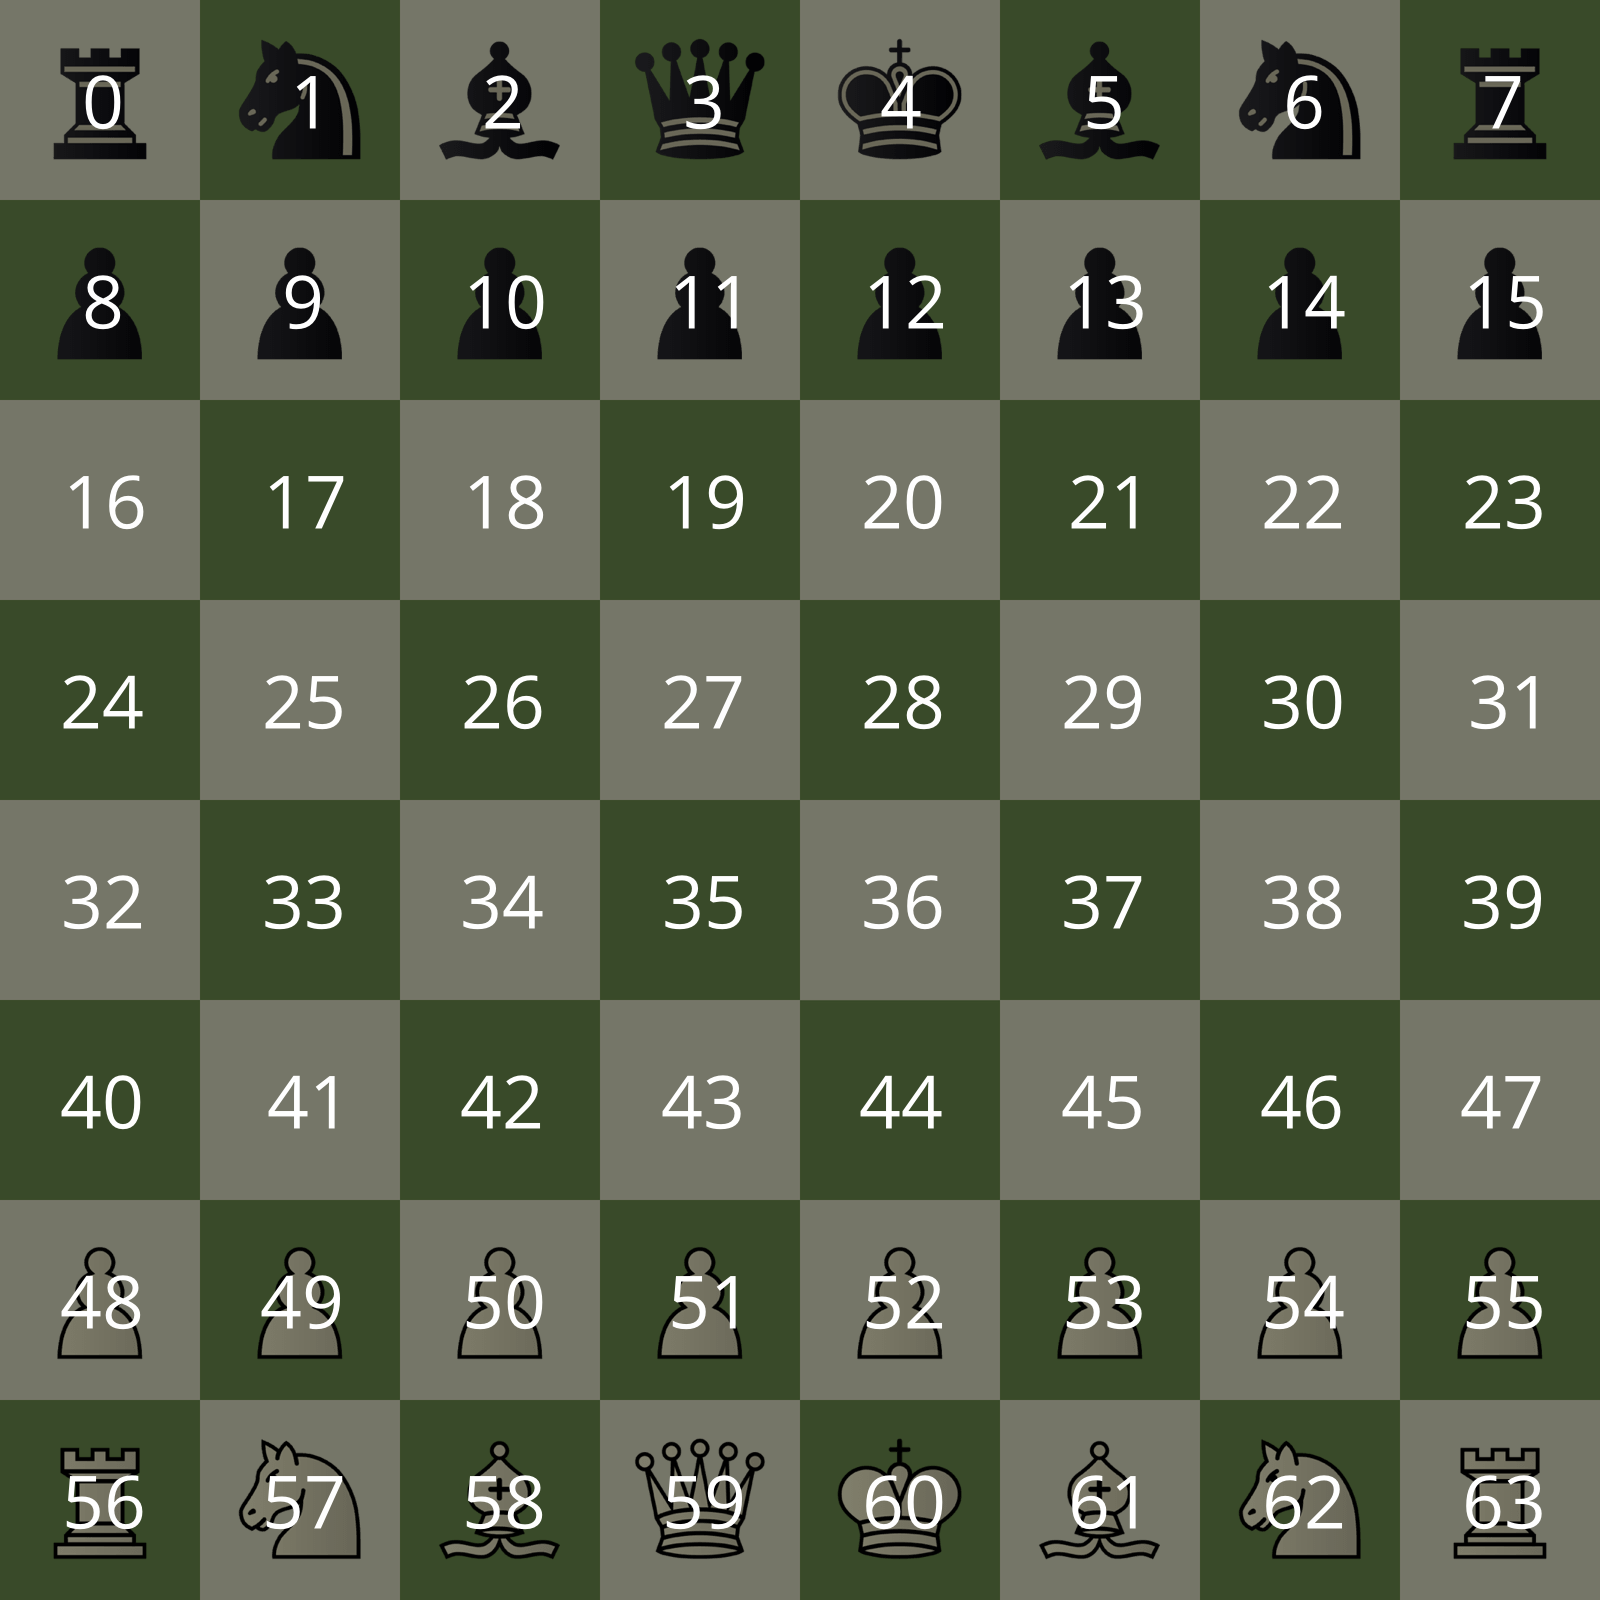
\includegraphics[scale=0.1]{board_indexed}
Detta är nödvändigt eftersom varje drag representeras på följande sätt, rutan som pjäsen börjar på, rutan som pjäsen slutar på, samt några extra bitars information som representerar vilken typ av drag det är. Rutorna representeras med

pub enum Direction {
    North = -8,
    West = -1,
    NorthWest = -9,
    NorthEast = -7,
    SouthWest = 7,
    SouthEast = 9,
    East = 1,
    South = 8,
}

Drag generingen är den delen av schackdatorn där användningen av bitboards blir som mest fördelaktig på grund av de operationer som effektiv kan manipulera bitboardsen. Schack har 6 olika pjäser som kan röra sig på olika sätt. Men för drag generingen är den generella principen samma, först använder vi lsb för att få positionen på brädet av en pjäs av en specifik typ. Detta låter oss slippa loopa igenom alla 64 bitar för att hitta pjäserna eftersom vi bara bryr oss om bitarna som är 1 och därmed har en pjäs. Därefter tar vi in en funktion som utifrån en startruta för en viss pjäs returnerar slutrutan för draget.


    for to in bitboard {
        let mov = mov(to);
        if legal(board, mov.from(), mov.to()) {
            moves.push(mov);
        }
      }

      För att generera alla hästdrag används följande funktion

fn generate_knight_moves(moves: &mut ArrayVec<Move, MAX_LEGAL_MOVES>, board: &Board) {
    let bitboard = board.piece_squares[Piece::new(PieceType::Knight, board.side)];

    for from in bitboard {
        let attack_bitboard = KNIGHT_ATTACK_MASKS[from] & !board.friendly_squares();
        add_moves_from_bitboard(&|to| Move::new(from, to, MoveType::Normal), moves, attack_bitboard, board);
    }
  }

  den har en for loop som letar igenom alla 1:or i bitboarden för alla hästar som tillhör spelar som ska göra ett drag.





\section{Sökning}
Minimax är ett algoritm som används för att bestämma poängen efter ett visst mängd drag för ett noll-summa spel vilket är vad schack är. Minimax är beroende av en evalueringsfunktion som ger ett heurestiskt mått på hur väl det går för spelarna. I mitt schackprogram använder jag en variation av minimax som kallas för negamax, vilket simplifierar koden genom att uttnytja följande faktum

\begin{math}
min(a,b)=max(-b,-a)
\end{math}

\subsection{Negamax}
Detta fungerar således evalueringsfunktionen returnerar ett värde som är relativt till sidan som gör draget--då större värden är bättre--vilket innebär att i negamax försöker både sidorna maximera evaluerings värde. 

Algoritmen fungerar genom att gå igenom ett träd av alla möjliga positioner till ett visst djup. Vi börjar vid brädets nuvarande positionen och genererar en lista av alla lagliga drag. För varje lagligt drag skapar vi en ny nod i trädet som representerar schackbrädets position efter att draget har gjorts. Vi får ett heurestiskt värde för en av dessa barnnoder genom att anropa negamax igen från barnnoden, vilket kommer att ge oss ett heurestiskt värde för hur bra positionen är för den nuvarande spelaren. 

Funktionen ger ett heurestiskt värde vid varje löv-nod som utgörs av de noder som nått det förutbestämda djupet eller som saknar lagliga drag, och noder som inte är löv-noder kommer ärva värdet värdet från det största värdet av sina barn noder. Funktionen kommer därmed rekursivt gå igenom trädet av alla drag på djupet först och varje nod kommer ärva det heurestiska värdet för det bässta draget i den nuvarande positionen.
Pseudokoden för algoritmet blir följande:

\begin{verbatim}
fn nega_max(depth ) {
    if (depth == 0) return evaluate();
    max = -oo;
    for (all moves)  {
        score = -negaMax(depth - 1);
        if(score > max)
            max = score;
    }
    return max;
}
\end{verbatim}

\subsection{Alpha-beta pruning}
Alpha-beta pruning är en förbättring på minimax som drastiskt kan minska antalet noder som behöver sökas. Principen utgår ifrån att vi sparar ett alfa och ett beta värde när vi söker, där alfa är det minsta poängen som den maximerande spelaren är garanterad, och beta är det största värdet som den minimerande spelaren är garanterad. Alfa får ett ursprungligt värde på -oo och beta oo. Dessa två värden är de sämsta möjliga som spelarna kan få, och när vi söker igenom trädet kommer vi uppdatera dessa. Efter vi har evaluerat värdet i en nod kollar vi ifall . Principen utgår ifrån att det bästa värdet som den maximerande spelaren kan få , a, är det sämsta värdet som den minimerande spelaren kan få, och tvärtom för b.

\subsection{Horisonteffekten}

Ett problem som dyker upp med vårt nuvarande sökalgoritm är en effekt som kallas för horisonteffekten. Eftersom vi har ett förutbestämt djup som vi söker till förekommer det situationer då det i lövnoden görs ett drag som har ett positivt vä. Ett exempel är ifall att det i en av lövnoderna görs ett drag där vits drottning tar en svart bonde, som i detta fallet blir positivt för vit. Problemet är att eftersom sökningen stannar vid detta djup kollar vi inte ifall det fanns en pjäs som skyddade den bonden och som nästa drag kommer ta drottningen. Detta kan lösas genom att vi inte stannar vid en nod som är instabil, dvs det finns drag som leder till en betydlig förändring i evalueringen. Det lättaste sättet att göra detta är att vi efter vår sökningen till en specifierad djuper, söker rekursivt genom alla drag som tar en annan pjäs. Detta fungerar relativt väl eftersom de drag som vanligast ger drastiska förändringar i evalueringen. Det finns fall där drag som inte tar pjäser ger drastiska förändringar i evalueringar, men dessa ignorerar vi att söka genom i vår horisontsökning eftersom det är svårt att bestämma det utan att göra draget, vilket skulle göra sökdjupet oändligt långt.

\subsection{Sortering av drag}

När vi söker igenom dragen spelar ordningen vi gör det i en stor roll. Detta beror på att alpha-beta pruningen kommer att bli mer effektiv om vi lyckas öka alfa och minska beta, dvs hitta bättre och bättre drag för de båda spelarna eftersom detta leder till fler alpha och beta cutoffs. Därmed är det viktigt att man sorterar dragen efter man har genererat dem. Det finns flera olika faktorer som kan uttnytjas för att få en effektiv sortering av drag. För att sortera dragen som i princip är en lista använder Rust något default sorteringsalgoritm där allting jag behöver skicka som argument är en funktion som tar in två drag och säger vilken som ska vara först i listan.

När man uttnytjar iterative deepening i sin sökmetod är en av de mest effektiva faktorerna för sorteringen ifall förra sökningens bästa linje innehåller det drag som man försöker sortera och vid rätt djup. Drag som man vid en tidigare sökning redan bestämt är bra har en väldigt hög chans att även vara bra vid ett djup högre, vilket är varför man vill söka dessa drag först.

En annan faktor följer tekniken MVV-LVA (Most valuable victim - Least valuable aggressor) som innebär att drag har högre chans att vara bättre dessto mer värdefull pjäsen som tas är och desto mindre värdefull pjäsen som tar den andra pjäsen är. Detta följer simpel logik då man vill ta mer värdefulla pjäser och när man tar en pjäs och om motståndarens pjäs är skyddad är det bättre att offra en mindre värdefull pjäs.
https://www.chessprogramming.org/MVV-LVA
Detta kan lätt implementeras i kod om man uttnytjar de förutbestämda material värdena för pjäserna genom att bara subtrahera pjäsen som blir tagens värde med pjäsen som tar den andra pjäsen.
let capture_score = captured_piece.piece_type().centipawns() - moving_piece.piece_type().centipawns();

Därefter är det bra att kolla transposition table


\subsection{Transposition Table}

När vi söker med minimax kommer vi att stötta på samma position senare i sökträdet i två separata sökningar även om dessa sökningar börjar med olika drag. Detta beror på att samma schackposition kan nås om man bara ändrar ordningen som man göra vissa drag i. När vi söker med negamax är det därmed användbart att hålla koll på alla positioner som vi har befunnit oss i samt, spara det djup och den evaluering som gavs till positionen i tidigare sökningar. Om vi stöter på positionen igen kan vi bara återanvända evalueringen som är sparat i transpositio ntablet. I koden implementeras Transposition table med en hashtable vars hashfunktion uttnytjar den tidigarenämnda zobrist hashing. Det finns en risk att zobrist hashingen är fel eftersom det inte är en perfekt hash funktion och det finns en risk för kollisioner, men

\begin{thebibliography}{9}

\end{thebibliography}

\end{document}
